\chapter{一元函数积分学}

物理问题中,有两类问题:1)求解一段非均匀物理量的累积;2)求解平均值。
积分用于解决这类问题。

本章先给出解决这类问题的方法——定积分。
由于从概念入手求解定积分过程繁琐,不具普遍性,所以随后通过微积分基本定理(牛顿莱布尼兹方程)引出不定积分,并讨论各种不定积分的求解方法,使得定积分的求解方法化。

对于定积分:
\begin{itemize}
    \item 充分理解定积分的概念、数学意义、几何意义和物理意义。
    \item 充分理解积分上限函数和原函数的概念。
    \item 掌握运用定积分求解工程问题(微元法)。
\end{itemize}

对于不定积分:
\begin{itemize}
    \item 理解不定积分的概念。
    \item 学会求解不定积分。
\end{itemize}

积分和微分是一个事物的两个方面,有着对立统一的矛盾关系。
学习积分要时时刻刻想着微分,对于积分中的每个概念和定理要思考在微分下的对应体。

\newpage
\section{一元函数积分学}

本节给出定积分的概念和意义。
定积分是一元函数积分学的目的,后续的牛顿莱布尼兹公式和不定积分是求解定积分的方法。

本节要点:
\begin{itemize}
    \item 理解定积分的概念和意义;
    \item 掌握用概念求解定积分。
\end{itemize}

%============================================================
\subsection{定积分的概念}

\begin{definition}[定积分]
设函数$f\left( x \right) $在$\left[ a,b \right] $上有界,将$\left[ a,b \right] $划分为$n$个小区间$a=x_0<x_1<x_2<...<x_{n-1}<x_n=b$,记每个小区间的长度$\Delta x_i=x_i-x_{i-1},i=1,2,...,n$,令最大长度$\lambda =\max \left\{ \Delta x_i \right\} $,在每个小区间$\left[ x_{i-1},x_i \right] $上任取一点$\xi _i\in \left[ x_{i-1},x_i \right] $,作和式$\sum_{i=1}^n{\left[ f\left( \xi _i \right) \cdot \Delta x_i \right]}$,若无论区间$\left[ a,b \right] $如何划分也无论点$\xi _i$如何选取,极限$\underset{\lambda \rightarrow 0}{\lim}\sum_{i=1}^n{\left[ f\left( \xi _i \right) \cdot \Delta x_i \right]}$存在且唯一,则称{\bf $f\left( x \right) $在$\left[ a,b \right] $上可积},该极限的值称为{\bf $f\left( x \right) $在$\left[ a,b \right] $上的定积分(definite integral)},记作$\int_a^b{f\left( x \right) dx}$,即:
\[
\int_a^b{f\left( x \right) dx}:=\underset{\lambda \rightarrow 0}{\lim}\sum_{i=1}^n{\left[ \xi _i\cdot \Delta x_i \right]}
\]
其中:
\begin{itemize}
    \item $x$:积分变量;
    \item $f\left( x \right) $:被积函数;
    \item $f\left( x \right) dx$:积分表达式,也称{\bf 微元};
    \item $a,b$:积分下限,积分上限;
    \item $\left[ a,b \right] $:积分区间。
\end{itemize}
\end{definition}

这个积分定义是黎曼(Riemann)给出的,通常称作{\bf 黎曼积分}。
黎曼积分存在的两个前提条件可以概括为闭区间和有限不连续。

\begin{tcolorbox}
黎曼可积的充要条件是勒贝格(Lebesgue)定理,即$f\left( x \right) $在$\left[ a,b \right] $上的不连续点组成的集合是一个零测度集。
如果不符合,则没有黎曼积分,需要扩充到勒贝格积分。
\end{tcolorbox}

注意,定积分概念里的两个“无关”:
\begin{itemize}
    \item 与区间划分方法无关,即$n$个小区间可以等分,也不可以不等分;
    \item 与区间点$\xi _i$的取法无关,即可以取在头、尾、中或者小区间内的任意一点。
\end{itemize}

\begin{tcolorbox}
一般的微积分教材里,将$\Delta x_i$称为“长度”。
但要特别注意,这个所谓的“长度”,是规定了方向的,是沿着{\it x}轴正方向,即$\Delta x_i=x_i-x_{i-1}$,不是$\Delta x_i=x_{i-1}-x_i$。
$\Delta x_i$必然是一个大于0的量。所以才有性质$\int_a^b{f\left( x \right) dx}=-\int_b^a{f\left( x \right) dx}$,细品!
\end{tcolorbox}

研究一函数在某一区间是否可积,关键在于判断和式极限
\[
\underset{\lambda \rightarrow 0}{\lim}\sum_{i=1}^n{\left[ f\left( \xi _i \right) \cdot \Delta x_i \right]}
\]
是否存在且唯一,步骤如下:
\begin{enumerate}
    \item 划分区间,通常等分;
    \item 取权重,通常取小区间的头或者尾;
    \item 求和式极限。
\end{enumerate}
所以定积分也是极限。
和求导一样,定积分也是对函数的一种运算,具体来说是对被积函数的一种运算,通过加权求和取极限这一过程得到另一个函数。
从集合角度,定积分是一个函数集合到另一个函数集合的映射。
这点在学习积分上限函数这个概念后细品!

%============================================================
\subsection{定积分的性质和定理}

区间性:
\begin{align*}
&a=b \quad \Rightarrow \quad \int_a^b{f\left( x \right) dx}=0 \\
&a\ne b \quad \Rightarrow \quad \int_a^b{f\left( x \right) dx}=-\int_b^a{f\left( x \right) dx}
\end{align*}

线性性:
\[
\int_a^b{\left[ mf\left( x \right) +ng\left( x \right) \right] dx}=m\int_a^b{f\left( x \right) dx}+n\int_a^b{g\left( x \right) dx}
\]

区间可加性:
\[
\int_a^b{f\left( x \right) dx}=\int_a^c{f\left( x \right) dx}+\int_c^b{f\left( x \right) dx}
\]

保号性:
\begin{align*}
&f\left( x \right) \geqslant 0 \quad \Rightarrow \quad \int_a^b{f\left( x \right) dx}\geqslant 0 \\
&f\left( x \right) \geqslant g\left( x \right) \quad \Rightarrow \quad \int_a^b{f\left( x \right) dx}\geqslant \int_a^b{g\left( x \right) dx}
\end{align*}

~

\begin{theorem}[连续可积定理]
$f\left( x \right) $在$\left[ a,b \right] $上连续$\Rightarrow f\left( x \right) $在$\left[ a,b \right] $上可积。
\end{theorem}

\begin{theorem}[有界可积定理]
$f\left( x \right) $在$\left[ a,b \right] $上有界,且只有有限个一类间断点$\Rightarrow f\left( x \right) $在$\left[ a,b \right] $上可积。
\end{theorem}

\begin{theorem}[估值定理]
设$M,m$分别是$f\left( x \right) $在$\left[ a,b \right] $上的最大值和最小值,则
\[
m\left( b-a \right) \leqslant \int_a^b{f\left( x \right) dx}\leqslant M\left( b-a \right)
\]
\end{theorem}

\begin{theorem}[积分中值定理]
若$f\left( x \right) $在$\left[ a,b \right] $上连续,则存在$\xi \in \left( a,b \right) $,使得
\[
\int_a^b{f\left( x \right) dx}=f\left( \xi \right) \left( b-a \right)
\]
\end{theorem}

估值定理和积分中值定理常用于定理的证明。
积分中值定理对应的微分中值定理中的拉格朗日定理,几何上表示必有矩形和曲边梯形面积相等,物理上必有均值点$\xi $及其均值$f\left( \xi \right) $。

\begin{tcolorbox}
细品后能发现,这些定理对曲线都要求不断。相比导数和微分,要求宽松了些。
\end{tcolorbox}

%============================================================
\subsection{定积分的代数意义}

在数学上,和式$\sum_{i=1}^n{\left[ f\left( \xi _i \right) \cdot \Delta x_i \right]}$可以看成加权和,每个累加项$\Delta x_i$加了权重$f\left( \xi _i \right) $后的代数和,整个和式也可以看成矩阵乘法:
\[
\sum_{i=1}^n{\left[ f\left( \xi _i \right) \cdot \Delta x_i \right]}=\left[ \begin{matrix}
	f\left( \xi _1 \right)&		f\left( \xi _2 \right)&		\cdots&		f\left( \xi _n \right)\\
\end{matrix} \right] \cdot \left[ \begin{array}{c}
	\Delta x_1\\
	\Delta x_2\\
	\vdots\\
	\Delta x_n\\
\end{array} \right]
\]
定积分就是当每个累加项都趋于无穷小,划分趋于无穷细、无穷多,情况下的这个代数和的极限。

\begin{tcolorbox}
从忽略高阶无穷小量的角度看,定积分的位置有点像微分。
\end{tcolorbox}

%============================================================
\subsection{定积分的几何意义}

考察曲线$y=f\left( x \right) $。
$f\left( \xi _i \right) \cdot \Delta x_i$是小区间的面积,和式$\sum_{i=1}^n{\left[ f\left( \xi _i \right) \cdot \Delta x_i \right]}$是所有小区间的面积的和,当小区间宽度越来越小时,和就越来越接近曲线下的面积。
当每个小区间的宽度都无穷小的时候,和式极限就是曲线下的面积。
所以几何上,定积分就是被积函数$y=f\left( x \right) $和{\it x}轴在积分区间$\left[ a,b \right] $里围成的面积。
\begin{figure}[h]
\centering
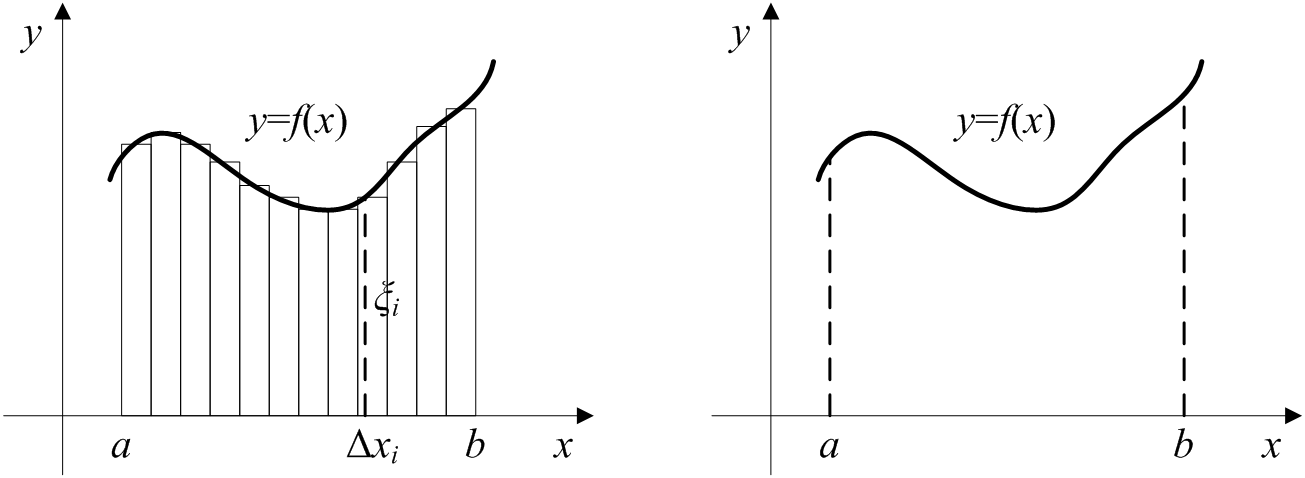
\includegraphics[height=3.5cm]{3.1.png}
\end{figure}

%============================================================
\subsection{定积分的物理意义}

物理量可以看成是很多分段小量的集合,每个小量又可以看成“加权小量”。
比方总路程$S$就可以看成很多分段$\Delta S$的累积,而$\Delta S$又是单位时间上平均速度的加权结果$\Delta S=\bar{v}\left( t \right) \cdot \Delta t$。
所以总路程为:
\[
S=\sum{\Delta S}=\sum{\left[ \bar{v}\left( t \right) \cdot \Delta t \right]}
\]
当单位时间$\Delta t\rightarrow 0$时,$\Delta t=dt$且有平均速度变成瞬时速度$\bar{v}\left( t \right) =v\left( t \right) $,有限段小路程变成无穷多段无穷小的路程$\Delta S=ds$,最终求和变成求积分:
\[
S=\int{ds}=\int{v\left( t \right) dt}
\]
这里需要注意的是,由于微元变量和变量本身有同样的量纲,所以$dt$的单位$t$和一样是秒,$ds=vdt$的单位是米。
% \begin{figure}[h]
% \centering
% 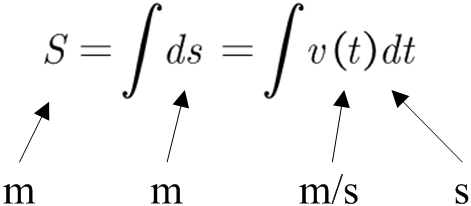
\includegraphics[height=2cm]{3.2.png}
% \end{figure}
所以,只要物理量是可以描述为加权积累效果的,都可以用定积分计算。






\newpage
\section{牛顿莱布尼兹公式}

上一节给出定积分的定义。
然而用定义求解定积分非常麻烦。
本节首先通过原函数的定义给出被积函数和导数运算之间的关系,然后介绍牛顿莱布尼兹公式,最后使用对被积函数求导逆运算求解定积分,大大简化了运算。

本节要点:
\begin{itemize}
    \item 掌握积分上限函数的概念;
    \item 掌握原函数的概念;
    \item 深入理解牛顿莱布尼兹公式。
\end{itemize}

%============================================================
\subsection{积分上限函数的概念}

\begin{definition}[积分上限函数]
如果对于区间$\left[ a,b \right] $上任意$x$,若存在定积分$\int_a^x{f\left( t \right) dt}$,则值必然唯一,且称它为{\bf $f\left( x \right) $在$\left[ a,b \right] $上的积分上限函数(accumulation function)},记为$F\left( x \right) $,即:
\[
F\left( x \right) :=\int_a^x{f\left( t \right) dt}
\]
\end{definition}

从几何上看,$F\left( x \right) $就是$f\left( x \right) $在$\left[ a,b \right] $上围成的面积,是自变量为$x$的函数,所以有时也称{\bf 面积函数}。

函数在给定区间的定积分是一个确定的数,而积分上限函数是对该函数的一种运算,得到的结果是另一个函数。
这点和导数和导函数类似。

%============================================================
\subsection{原函数的概念}

\begin{definition}[原函数]
若函数$f\left( x \right) $在$\left[ a,b \right] $上连续,则函数$F\left( x \right) $在$\left[ a,b \right] $上可导,且$F'\left( x \right) =f\left( x \right) $,称$F\left( x \right) $为{\bf $f\left( x \right) $在$\left[ a,b \right] $上的一个原函数}。
\end{definition}

\begin{proof}
即证明$F'\left( x \right) =f\left( x \right) $,从导数的定义出发,结合积分中值定理,有:
\begin{align*}
F'\left( x_0 \right) &=\underset{\Delta x\rightarrow 0}{\lim}\frac{\int_a^{x_0+\Delta x}{f\left( d \right) dt}-\int_a^{x_0}{f\left( d \right) dt}}{\Delta x} \\
&=\underset{\Delta x\rightarrow 0}{\lim}\frac{\int_{x_0}^{x_0+\Delta x}{f\left( d \right) dt}}{\Delta x}=\underset{\Delta x\rightarrow 0}{\lim}\frac{f\left( \xi \right) \cdot \Delta x}{\Delta x}
\end{align*}
当$\Delta x\rightarrow 0$时,有$\xi \rightarrow x_0$,从而:
\[
F'\left( x_0 \right) =\underset{\Delta x\rightarrow 0}{\lim}\frac{f\left( \xi \right) \cdot \Delta x}{\Delta x}=f\left( x_0 \right)
\]
\end{proof}

注意,“原函数”是“积分上限函数”的子集。
“积分上限函数”不要求被积函数连续,而“原函数”需要被积函数具备连续性。

$F\left( x \right) =\int_a^x{f\left( t \right) dt}$仅表示$f\left( x \right) $可积性。
如果$f\left( x \right) $不连续,那只要满足区间内有界,且一类间断点有限个,依然可积(即满足“有界可积定理”),只是$F\left( x \right) $在间断点是不可导的。
而一旦$f\left( x \right) $满足连续性要求,则除了满足上式,还满足$F'\left( x \right) =f\left( x \right) $,即整个$\left[ a,b \right] $上可导。

至此,对于连续函数$f\left( x \right) $,我们找到了计算定积分(数值计算)和函数求导(函数运算)之间的关系。
如果$F\left( x \right) $的导数正好是$f\left( x \right) $,则$F\left( x \right) $就是$f\left( x \right) $的定积分,即:
\begin{align*}
&\text{微分形式表达:} F'\left( x \right) =f\left( x \right) \\
&\text{积分形式表示:} F\left( x \right) =\int_a^x{f\left( t \right) dt}
\end{align*}

在积分定理中,原函数和被积函数唯一的联系是$x$,且$x$必然出现在积分上限(如果是积分下限,可以对调换到上限,如果同时出现在上下限,必须通过区间可加性定理拆分成上下限)。

%============================================================
\subsection{积分复合函数的求导}

\begin{definition}[积分复合函数]
当原函数的积分上限以函数的形式出现时,如:
\[
F\left( x \right) =\int_a^{\varphi \left( x \right)}{f\left( t \right) dt}
\]
称为{\bf 积分复合函数}。
对于此类函数,根据复合函数求导法则,有:
\[
F'\left( x \right) =\left[ \frac{d}{d\varphi}\int_a^{\varphi \left( x \right)}{f\left( t \right) dt} \right] \cdot \frac{d\varphi}{dx}=f\left[ \varphi \left( x \right) \right] \cdot \varphi '\left( x \right)
\]
\end{definition}

~

\begin{example}
已知$F\left( x \right) =\int_a^{x^2+1}{\sin \left( t+1 \right) dt}$,求$F'\left( x \right) $。
\end{example}

解:
\[
F'\left( x \right) =f\left[ \varphi \right] \cdot \varphi '=\sin \left[ \left( x^2+1 \right) +1 \right] \cdot \left( x^2+1 \right) '=2x\sin \left( x^2+2 \right)
\]

~

\begin{example}
求$\underset{x\rightarrow 0}{\lim}\frac{\int_{\cos x}^1{e^{-t^2}dt}}{x^2}$。
\end{example}

解:

可用洛必达法则求解:
\begin{align*}
&\because \left( \int_{\cos x}^1{e^{-t^2}dt} \right) '=f\left[ \varphi \right] \cdot \varphi '=-e^{-\cos ^2x}\cdot \left( -\sin x \right) =\sin x\cdot e^{-\cos ^2x} \\
&\therefore \underset{x\rightarrow 0}{\lim}\frac{\int_{\cos x}^1{e^{-t^2}dt}}{x^2}=\underset{x\rightarrow 0}{\lim}\frac{\sin x\cdot e^{-\cos ^2x}}{2x}=\frac{1}{2}\underset{x\rightarrow 0}{\lim}e^{-\cos ^2x}=\frac{1}{2e}
\end{align*}

%============================================================
\subsection{微积分基本定理}

\begin{theorem}[微积分基本定理]
如果$F\left( x \right) $是连续函数$f\left( x \right) $在$\left[ a,b \right] $上的一个原函数,即$F'\left( x \right) =f\left( x \right) $,则:
\[
\int_a^b{f\left( x \right) dx}=F\left( b \right) -F\left( a \right)
\]
该公式称为{\bf 牛顿—莱布尼兹(Newton-Leibniz)公式}。
\end{theorem}

牛顿莱布尼兹公式告诉我们,只要是连续函数,则在一个区域内的积分只跟其两端有关。
更抽象一点,对区域的考察可以变成对其边界的考察。
学完多元函数微积分(特别是统一公式)后,再回来细品牛顿莱布尼兹公式!

%============================================================
\subsection{再看定积分的几何意义}

假设函数$y=f\left( x \right) $在区间$\left[ a,b \right] $可导,已知$x$的变化量$\Delta x$,如何确定$\Delta y$。
首先,将区间$\left[ a,b \right] $化为$n$个小区间,运用微分的概念每个小区间可以认为有:
\[
dy=y'\cdot dx
\]
\begin{figure}[h]
\centering
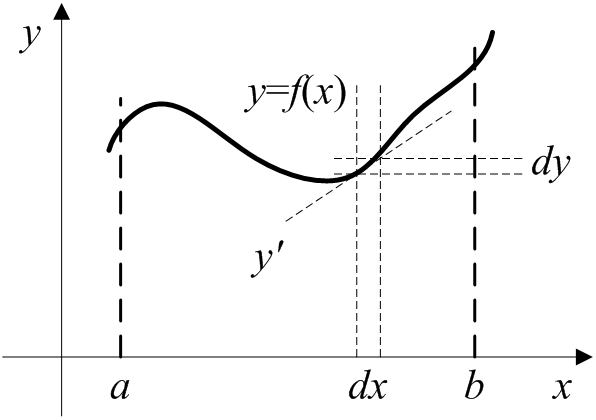
\includegraphics[height=3.5cm]{3.3.png}
\end{figure}

再将这些小区间上的微增量$dy$累积,就能得到$\Delta y$:
\[
\Delta y=\int_a^b{dy}=\int_a^b{y'\cdot dx}
\]
这里,对于每个小区间,$y'$可以认为是$dx$的权重,且$y'$有正有负。
几何上这个权重使得该段对$y$的变化量贡献也有正有负。
最终,$\Delta y$由各个$dy$累积得到。

%============================================================
\subsection{再看定积分的物理意义}

以变速运动为例。
从总体性考察,在一个范围内走过的路程$S\left( t \right) $为过程中的每个小微元$ds\left( t \right)$累积而成:
\[
S\left( t \right) =\int_0^t{ds\left( t \right)}
\]
从局部性考察,极端的时间内走过的路程和时间的比为一个固定的值:
\[
v\left( t \right) =\frac{ds\left( t \right)}{dt}
\]
结合上述两式:
\[
S\left( t \right) =\int_0^t{ds\left( t \right)}=\int_0^t{v\left( t \right) \cdot dt}
\]

\begin{tcolorbox}
“所谓的积分,就是由微分累积而成,所谓的微分,就是积分的局部化分析。”
这就是“教材\cite{book2}”中始终贯穿的微积分的矛盾统一论。
\end{tcolorbox}

%============================================================
\subsection{再看中值定理}

将微分中值定理(拉格朗日定理)和积分中值定义对比看。

用牛顿莱布尼兹公式,拉格朗日定理可以写为:
{\bf 设$F\left( x \right) $在$\left[ a,b \right] $连续,在$\left( a,b \right) $可导,则必有$\xi \in \left( a,b \right) $,使得$f\left( \xi \right) =F'\left( \xi \right) =\frac{F\left( b \right) -F\left( a \right)}{b-a}$。}

对比积分中值定理:
{\bf 若$f\left( x \right) $在$\left[ a,b \right] $上连续,则必有$\xi \in \left( a,b \right) $,使得$\int_a^b{f\left( x \right) dx}=f\left( \xi \right) \left( b-a \right)$。}

可见,两个中值定理描述的是一件事,只不过从两个方面描述而已。
这也反映出微分和积分是对立统一的。






\newpage
\section{半章小结}

至此,导数、微分、定积分三者关系确立:
\begin{itemize}
    \item 导数是整个微积分的基础;
    \item 微分定理给出了微增量和导数的关系$df\left( x \right) =f'\left( x \right) \cdot dx$;
    \item 牛顿莱布尼兹公式给出了累积量和导数的关系$\int_a^b{f\left( x \right) dx}=F\left( b \right) -F\left( a \right)$。
\end{itemize}

微分和积分所表达的是一个事物的两个方面,这个事物就是光滑。
微分是从“变化”的角度看光滑,积分是从“累积”的角度看光滑。
所以,一般地,微分里的概念和定理在积分里都会有对应的表达。
也正是微分和积分的这种对立统一关系,使得在解决实际问题时才有“微元法”这个普遍意义上的数学方法。

至此,微积分的基本思想建立完成。
我们需要从“微”和“积”两个方面理解微分和积分的对立,更要从逻辑论和认识论上理解微分和积分这一对矛盾体的对立统一。
这对矛盾体统一在光滑,是光滑衍生出来的在微和积方面的两个对立。






\newpage
\section{不定积分}

本节给出不定积分这个概念,这个概念完全是为了求解定积分,将定积分的求解过程中的求原函数步骤独立出来研究,讨论各种方法(换元法、凑微法、部分积分法等)。

本节要点:
\begin{itemize}
    \item 掌握不定积分的计算方法。
\end{itemize}

%============================================================
\subsection{不定积分的概念}

\begin{definition}[不定积分]
若某区间上$F\left( x \right) $是$f\left( x \right) $的一个原函数,则$f\left( x \right) $所有原函数的一般表达式$F\left( x \right) +C$称为{\bf $f\left( x \right) $的不定积分(indefinite function)},记为$\int{f\left( x \right) dx}$,即:
\[
\int{f\left( x \right) dx}:=F\left( x \right) +C
\]
其中:
\begin{itemize}
    \item $x$:积分变量;
    \item $f\left( x \right) $:被积函数;
    \item $f\left( x \right) dx$:积分表达式。
\end{itemize}
\end{definition}

定积分可以理解为不定积分在一段区间内的变化量。

%============================================================
\subsection{不定积分的几何意义}

\begin{figure}[h]
\centering
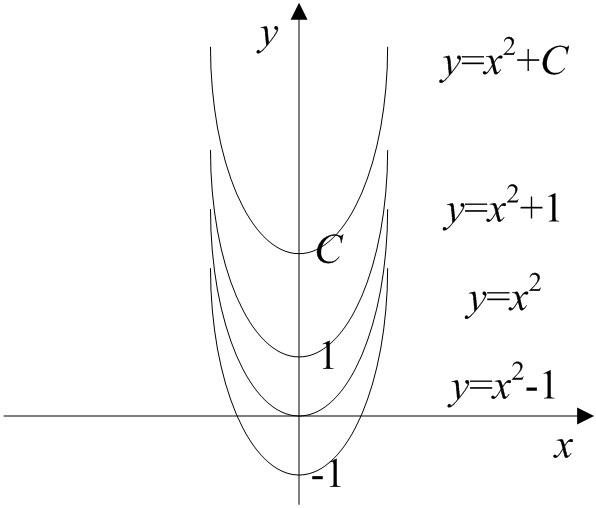
\includegraphics[height=4cm]{3.4.png}
\end{figure}

切线符合$y=x^2$的所有曲线的集合。

%============================================================
\subsection{不定积分的性质}

互逆运算:
\begin{align*}
&\left[ \int{f\left( x \right) dx} \right] '=f\left( x \right) \\
&\int{F'\left( x \right) dx}=F\left( x \right) +C
\end{align*}

线性性:
\[
\int{\left[ mf\left( x \right) +ng\left( x \right) \right] dx}=m\int{f\left( x \right) dx}+n\int{g\left( x \right) dx}
\]

\begin{tcolorbox}
线性性对应着导数运算中的$\left( f\pm g \right) '=f'\pm g'$。
\end{tcolorbox}

%============================================================
\subsection{不定积分计算方法}

{\bf 换元法(凑微分法)}:设$u=u\left( x \right) $具有连续导数,$F\left( u \right) $是$f\left( u \right) $的一个原函数,则:
\[
\int{f\left( u \right) u'\left( x \right) dx}=\int{f\left( u \right) du}=F\left( u \right) +C=F\left[ u\left( x \right) \right] +C
\]

\begin{tcolorbox}
线性性对应着导数运算中的$\frac{dy}{dx}=\frac{dy}{du}\cdot \frac{du}{dx}$。
\end{tcolorbox}

常用换元公式:
\begin{align*}
&\int{f\left( ax+b \right) dx}=\frac{1}{a}\int{f\left( ax+b \right) d\left( ax+b \right)} \quad a\ne 0 \\
&\int{f\left( x^a \right) x^{a-1}dx}=\frac{1}{a}\int{f\left( x^a \right) d\left( x^a \right)} \quad a\ne 0 \\
&\int{f\left( e^x \right) e^xdx}=\int{f\left( e^x \right) d\left( e^x \right)} \\
&\int{f\left( \ln x \right) \frac{1}{x}dx}=\int{f\left( \ln x \right) d\left( \ln x \right)} \\
&\int{\frac{\varphi '\left( x \right)}{\varphi \left( x \right)}dx}=\int{\frac{1}{\varphi \left( x \right)}d\varphi \left( x \right)}=\ln \left| \varphi \left( x \right) \right|+C
\end{align*}

~

{\bf 部分积分法}:设$u\left( x \right) ,v\left( x \right) $都具有连续导数,则:
\[
\int{uv'dx}=uv-\int{u'vdx} \quad \text{或写成} \quad \int{udv}=uv-\int{vdu}
\]

\begin{tcolorbox}
部分积分法和微分中的导数运算法则对应,$\left( fg \right) '=f'g+fg'$。
\end{tcolorbox}

%============================================================
\subsection{基本积分公式}

\begin{align*}
&\int{0dx}=C \\
&\int{x^adx}=\frac{1}{a+1}x^{a+1}+C \quad a\ne -1 \\
&\int{\frac{1}{x}dx}=\ln \left| x \right|+C \\
&\int{a^xdx}=\frac{a^x}{\ln a}+C \quad a>0,a\ne -1 \\
&\int{e^xdx}=e^x+C \\
&\int{\cos xdx}=\sin x+C \\
&\int{\sin xdx}=-\cos x+C \\
&\int{\sec ^2xdx}=\tan x+C \\
&\int{\csc ^2xdx}=-\cot x+C \\
&\int{\sec x\tan xdx}=\sec x+C \\
&\int{\csc x\cot xdx}=-\csc x+C \\
&\int{\frac{1}{\sqrt{1-x^2}}dx}=\mathrm{arc}\sin x+C \\
&\int{\frac{1}{1+x^2}dx}=\mathrm{arc}\tan x+C
\end{align*}






\newpage
\section{反常积分}

定积分的要求是积分区间是有限区间,被积函数是有界函数。
如果这两条中任何一条不满足,定积分的概念就不适用。

本节要点:
\begin{itemize}
    \item 了解反常积分;
    \item 了解伽马函数和贝塔函数。
\end{itemize}

%============================================================
\subsection{无穷区间上的反常积分}

\begin{definition}[无穷型反常积分]
设$f\left( x \right) $在无穷区间$\left[ a,+\infty \right] $上连续,则称极限$\underset{b\rightarrow +\infty}{\lim}\int_a^b{f\left( x \right) dx},b>a$为{\bf $f\left( x \right) $在无穷区间$\left[ a,+\infty \right] $上的反常积分},记为$\int_a^{+\infty}{f\left( x \right) dx}$,即:
\[
\int_a^{+\infty}{f\left( x \right) dx}:=\underset{b\rightarrow +\infty}{\lim}\int_a^b{f\left( x \right) dx} \qquad b>a
\]
如果该极限存在,称该{\bf 反常积分收敛},反之称该{\bf 反常积分发散}。

同理,设$f\left( x \right) $在无穷区间$\left[ -\infty ,b \right] $上连续,则称$\underset{a\rightarrow -\infty}{\lim}\int_a^b{f\left( x \right) dx},b>a$为{\bf $f\left( x \right) $在无穷区间$\left[ -\infty ,b \right] $上的反常积分},记为$\int_{-\infty}^b{f\left( x \right) dx}$,即:
\[
\int_{-\infty}^b{f\left( x \right) dx}:=\underset{a\rightarrow -\infty}{\lim}\int_a^b{f\left( x \right) dx} \qquad b>a
\]

综合以上,设$f\left( x \right) $在$\left[ -\infty ,+\infty \right] $上连续,定义{\bf $f\left( x \right) $在$\left[ -\infty ,+\infty \right] $上的反常积分}为:
\[
\int_{-\infty}^{+\infty}{f\left( x \right) dx}:=\int_{-\infty}^0{f\left( x \right) dx}+\int_0^{+\infty}{f\left( x \right) dx}
\]
\end{definition}

%============================================================
\subsection{无界函数的反常积分}

\begin{definition}[开区间型反常积分]
设$f\left( x \right) $在$\left[ a,b \right) $上连续,在$b$点的左邻域内无界,则称极限$\underset{\varepsilon \rightarrow 0^+}{\lim}\int_a^{b-\varepsilon}{f\left( x \right) dx}$为{\bf $f\left( x \right) $在$\left[ a,b \right) $上的反常积分}:
\[
\int_a^b{f\left( x \right) dx}:=\underset{\varepsilon \rightarrow 0^+}{\lim}\int_a^{b-\varepsilon}{f\left( x \right) dx}
\]
如果该极限存在,称该{\bf 反常积分收敛},反之称该{\bf 反常积分发散}。

同理,设$f\left( x \right) $在$\left( a,b \right] $上连续,在$a$点的右邻域内无界,则称极限$\underset{\varepsilon \rightarrow 0^+}{\lim}\int_{a+\varepsilon}^b{f\left( x \right) dx}$为{\bf $f\left( x \right) $在$\left( a,b \right] $上的反常积分}:
\[
\int_a^b{f\left( x \right) dx}:=\underset{\varepsilon \rightarrow 0^+}{\lim}\int_{a+\varepsilon}^b{f\left( x \right) dx}
\]

综合以上,设$f\left( x \right) $在$\left[ a,b \right] -\left\{ c \right\} $上连续,在$c$点的某邻域内无界,定义{\bf $f\left( x \right) $在$\left[ a,b \right] $上的反常积分}为:
\[
\int_a^b{f\left( x \right) dx}:=\int_a^c{f\left( x \right) dx}+\int_c^b{f\left( x \right) dx}
\]
\end{definition}

反常积分不是定积分,虽然采用定积分的符号,而是定积分的极限。
无穷区间的反常积分是{\it x}轴上无限,无界函数的反常积分对应几何上是{\it y}轴上的无限。

%============================================================
\subsection{伽马函数和贝塔函数}

\begin{definition}[伽马函数($\Gamma $函数)]
\[
\Gamma \left( x \right) :=\int_0^{+\infty}{e^{-t}t^{x-1}dt} \qquad x>0
\]
\end{definition}

$\Gamma $函数的性质,证明略:
\begin{itemize}
    \item $\Gamma \left( 1 \right) =1$;
    \item $\Gamma \left( x \right) =\left( x-1 \right) \Gamma \left( x-1 \right) $,特别的取整数$n$时有$\Gamma \left( n \right) =\left( n-1 \right) !$;
    \item $\Gamma \left( x \right) \Gamma \left( 1-x \right) =\frac{\pi}{\sin \pi x}$;
    \item $\underset{x\rightarrow 0^+}{\lim}\Gamma \left( x \right) =+\infty $;
    \item $\Gamma \left( \frac{1}{2} \right) =\sqrt{\pi}$。
\end{itemize}

\begin{definition}[贝塔函数($\mathrm{B}$函数)]
\[
\mathrm{B}\left( \alpha ,\beta \right) :=\int_0^1{x^{\alpha -1}\left( 1-x \right) ^{\beta -1}dx} \qquad \alpha ,\beta \in \left( 0,1 \right)
\]
\end{definition}

$\mathrm{B}$函数的性质,证明略。
\begin{itemize}
    \item $\mathrm{B}\left( 1,1 \right) =1$;
    \item $\mathrm{B}\left( \alpha ,\beta \right) =\mathrm{B}\left( \beta ,\alpha \right) $,对称性;
    \item $\mathrm{B}\left( \alpha +1,\beta +1 \right) =\frac{\alpha \beta}{\left( \alpha +\beta \right) \left( \alpha +\beta +1 \right)}\mathrm{B}\left( \alpha ,\beta \right) $,特别地,取整数$m,n$时有$\mathrm{B}\left( m,n \right) =\frac{\left( m-1 \right) !\left( n-1 \right) !}{\left( m+n-1 \right) !}$;
    \item $\mathrm{B}\left( \alpha ,\beta \right) =\frac{\Gamma \left( \alpha \right) \Gamma \left( \beta \right)}{\Gamma \left( \alpha +\beta \right)}$。
\end{itemize}

\begin{tcolorbox}
$\Gamma $函数和$\mathrm{B}$函数将以往以自然数为定义域的函数(如阶乘)扩展到了实数域,所以特别在数理统计有着广泛的应用。
\end{tcolorbox}





\newpage
\section{定积分的应用}

对于非均匀分布的物理量的累积,可以用定积分求解,关键是建立积分表达式——微元法。
微元法把物理量分割成一个个小量——微元,每个微元内近似分布均匀,对这个分布均匀的微元列出表达式,最后积分。

本节要点:
\begin{itemize}
    \item 通过3个例子体会定积分的应用及使用方法;
    \item 了解平均值和均方根值的概念。
\end{itemize}

\begin{tcolorbox}
注意,微元法中,我们先微分再积分,体会这个矛盾统一体。
\end{tcolorbox}

%============================================================
\subsection{变力作功}

\begin{example}
假设弹簧的胡克系数$k$,从放松状态拉长$l$,需做多少功?
\end{example}

解:

根据功的定义$W=F\cdot S$,对拉长微元$dx$内可以认为力$F\left( x \right) =kx$不变,该拉长微元下功的微元$dW=F\left( x \right) dx=kx\cdot dx$,于是,整体作功:
\[
W=\int_0^l{dW}=\int_0^l{kx\cdot dx}=\left. \frac{1}{2}kx^2 \right|_{0}^{l}=\frac{1}{2}kl^2
\]

%============================================================
\subsection{一维物体引力}

\begin{example}
小球质量$m$,均匀细长杆质量$M$、长$L$、重量均匀且密度为$\mu $,小球位于细长杆延长线,距细长杆$d$,求小球受到的引力。
\begin{figure}[h]
\centering
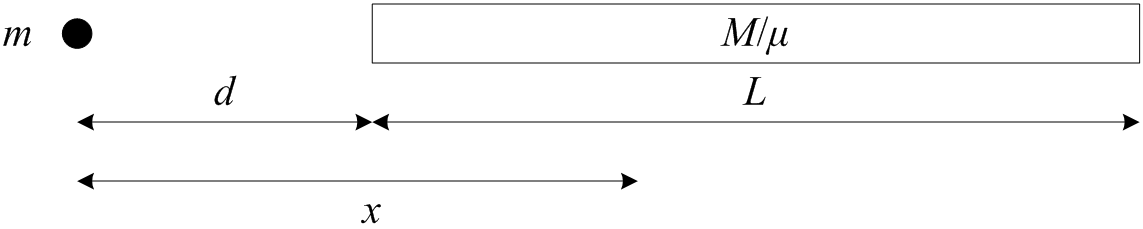
\includegraphics[height=1.5cm]{3.5.png}
\end{figure}
\end{example}

解:

小球可以视为质点,但细长杆不行,根据引力方程,假设细长杆的一个微元对小球的引力可以视为质点,则引力微元$dF=G\frac{m\cdot \mu dx}{x^2}$,整体引力:
\begin{align*}
F&=\int_d^{d+L}{G\frac{m\cdot \mu dx}{x^2}}=Gm\mu \int_d^{d+L}{\frac{1}{x^2}\cdot dx} \\
&=Gm\mu \left( \left. -\frac{1}{x} \right|_{d}^{d+L} \right) =Gm\mu \left( \frac{1}{d}-\frac{1}{d+L} \right)
\end{align*}

%============================================================
\subsection{第二宇宙速度}

\begin{example}
求第二宇宙速度,即脱离地球引力范围的最小速度。
\end{example}

解:

假设地球质量$M$,物体质量$m$,地球半径$R$,脱离地球引力范围即相当于飞至无限远。
结合能量守恒定律,物体飞至无限远引力做功即物体的初动能:
\[
\frac{1}{2}{mv_0}^2=\int_R^{+\infty}{F\left( r \right) dr}=\int_R^{+\infty}{G\frac{Mm}{r^2}dr}
\]
该问题从数学上看是一个无穷区间上的反常积分:
\begin{align*}
&\because \int_R^{+\infty}{G\frac{Mm}{r^2}dr}=GMm\left( \left. -\frac{1}{r} \right|_{R}^{+\infty} \right) =\frac{GMm}{R} \\
&\therefore v_0=\sqrt{\frac{2GM}{R}}=\sqrt{2gR}\approx 11.2\mathrm{km}/\mathrm{s}
\end{align*}
物体的初速度11.2km/s,即为第二宇宙速度。

%============================================================
\subsection{函数的平均值和均方根值}

之前我们讨论了离散量的算术平均值:
\[
\bar{x}=\frac{x_1+x_2+\cdots +x_n}{n}
\]
如果是连续量,如电流、功率,就涉及连续函数的平均值。

\begin{definition}[函数的平均值]
设函数$f\left( x \right) $在$\left[ a,b \right] $上连续,将$\left[ a,b \right] $等分为$n$个小区间$a=x_0<x_1<x_2<...<x_{n-1}<x_n=b$,记每个小区间的长度$\Delta x_i=\frac{b-a}{n}$,我们可以用:
\[
\frac{f\left( x_1 \right) +f\left( x_2 \right) +\cdots +f\left( x_n \right)}{n}=\frac{1}{n}\sum_{i=1}^n{f\left( x_i \right)}
\]
近似描述平均值,如果当$n\rightarrow \infty $时该和式有极限,我们就称该极限为{\bf 函数$f\left( x \right) $在$\left[ a,b \right] $上的平均值},记作$\bar{y}$,即:
\begin{align*}
\bar{y}:&=\underset{n\rightarrow \infty}{\lim}\frac{1}{n}\sum_{i=1}^n{f\left( x_i \right)}=\underset{n\rightarrow \infty}{\lim}\sum_{i=1}^n{\frac{f\left( x_i \right)}{n}} \\
&=\underset{n\rightarrow \infty}{\lim}\sum_{i=1}^n{\left[ f\left( x_i \right) \cdot \frac{\Delta x_i}{b-a} \right]}=\frac{1}{b-a}\underset{n\rightarrow \infty}{\lim}\sum_{i=1}^n{\left[ f\left( x_i \right) \cdot \Delta x_i \right]} \\
&=\frac{1}{b-a}\int_a^b{f\left( x \right) dx}
\end{align*}
\end{definition}

\begin{definition}[函数的均方根值]

若函数$f\left( x \right) $在$\left[ a,b \right] $上连续,我们称如下积分为{\bf 函数$f\left( x \right) $在$\left[ a,b \right] $上的均方根值},常记作RMS(Root Mean Square),即:
\[
RMS:=\sqrt{\frac{1}{b-a}\int_a^b{f^2\left( x \right) dx}}
\]
\end{definition}

物理上,我们通常用平均值表示一个物理量一段时间内的平均值,特别是周期物理量,用均方根值表示物理量的有效值。

~

\begin{example}
若交流电的电流$I\left( t \right) =I_m\sin \omega t$,$I_m$为峰值,计算在电阻$R$上的平均功率和有效电流。
\end{example}

解:

交流电的平均功率可以计算在一个周期$T=2\pi /\omega $内的功率的平均值,如下:
\begin{align*}
&\because P\left( t \right) =I^2\left( t \right) R=\left( I_m\sin \omega t \right) ^2R \\
&\therefore \bar{P}=\frac{1}{T}\int_0^T{P\left( t \right) dt}=\frac{\omega}{2\pi}\int_0^{2\pi /\omega}{\left( I_m\sin \omega t \right) ^2R\cdot dt}=\frac{1}{2}{I_m}^2R
\end{align*}
有效电流采用均方根值计算方式:
\[
\sqrt{\frac{1}{T}\int_0^T{I^2\left( t \right) \cdot dt}}=\sqrt{\frac{\omega}{2\pi}\int_0^{2\pi /\omega}{\left( I_m\sin \omega t \right) ^2\cdot dt}}=\frac{1}{\sqrt{2}}I_m
\]






\newpage
\section{本章小结}

本章介绍了积分。
其中,定积分是明确具备工程或物理意义的数学概念,能用于解决实际问题的数学工具。
但依照定积分的定义进行计算时,计算量非常大。
所以我们通过牛顿莱布尼兹公式引出不定积分的概念,给出了计算定积分的一个系统的方法,极大方便了计算。

\begin{itemize}
    \item 定积分:着重在理解其定义的几何、工程、物理等意义。
    \item 不定积分:学习和掌握各种求解不定积分的方法,不需要熟练,不定积分的计算是为后续微分方程准备的,其公式推导有现成软件。
\end{itemize}






\newpage
\section{习题}

\begin{exercise}
计算下列导数和极限:
\begin{enumerate}
    \item $\frac{d}{dx}\int_0^{x^2}{\sqrt{1+t^2}dt}$
    \item $\frac{d}{dx}\int_{\sin x}^{\cos x}{\cos \left( \pi t^2 \right) dt}$
    \item $\underset{x\rightarrow 0}{\lim}\frac{\int_0^x{\cos t^2dt}}{x}$
    \item $\underset{x\rightarrow +\infty}{\lim}\frac{\left( \int_0^x{e^{t^2}dt} \right) ^2}{\int_0^x{e^{2t^2}dt}}$
\end{enumerate}
\end{exercise}

解:

1.
\[
\frac{d}{dx}\int_0^{x^2}{\sqrt{1+t^2}dt}=\sqrt{1+\left( x^2 \right) ^2}\cdot \left( x^2 \right) '=2x\sqrt{1+x^4}
\]

2.
\begin{align*}
&\frac{d}{dx}\int_{\sin x}^{\cos x}{\cos \left( \pi t^2 \right) dt} \\
&=\frac{d}{dx}\int_{\sin x}^0{\cos \left( \pi t^2 \right) dt}+\frac{d}{dx}\int_0^{\cos x}{\cos \left( \pi t^2 \right) dt} \\
&=-\cos \left( \pi \sin ^2x \right) \cdot \cos x-\cos \left( \pi \cos ^2x \right) \cdot \sin x
\end{align*}

3.
\[
\underset{x\rightarrow 0}{\lim}\frac{\int_0^x{\cos t^2dt}}{x}=\underset{x\rightarrow 0}{\lim}\frac{\cos x^2\cdot 1}{1}=1
\]

4.
\begin{align*}
\underset{x\rightarrow +\infty}{\lim}\frac{\left( \int_0^x{e^{t^2}dt} \right) ^2}{\int_0^x{e^{2t^2}dt}}&=\underset{x\rightarrow +\infty}{\lim}\frac{2\left( \int_0^x{e^{t^2}dt} \right) \cdot e^{x^2}}{e^{2x^2}} \\
&=2\underset{x\rightarrow +\infty}{\lim}\frac{\int_0^x{e^{t^2}dt}}{e^{x^2}}=2\underset{x\rightarrow +\infty}{\lim}\frac{e^{x^2}\cdot 1}{2xe^{x^2}}=0
\end{align*}

\begin{tcolorbox}
主要是理解含积分复合函数的求导。
\end{tcolorbox}

~

\begin{exercise}
若方程$\int_0^y{e^tdt}+\int_0^x{\cos tdt}=0$确定函数$y=f\left( x \right) $,求$\frac{dy}{dx}$。
\end{exercise}

解:

大体思路是隐函数和积分复合函数的混合体,令隐函数$F\left( x,y \right) =\int_0^y{e^tdt}+\int_0^x{\cos tdt}=0$,则:
\begin{align*}
&\because \begin{cases}
	F_x=\frac{d}{dx}\left( \int_0^y{e^tdt}+\int_0^x{\cos tdt} \right) =e^y\cdot 0+\cos x\cdot 1=\cos x\\
	F_y=\frac{d}{dy}\left( \int_0^y{e^tdt}+\int_0^x{\cos tdt} \right) =e^y\cdot 1+\cos x\cdot 0=e^y\\
\end{cases} \\
&\therefore \frac{dy}{dx}=-\frac{F_x}{F_y}=-\frac{\cos y}{e^y}
\end{align*}

~

\begin{exercise}
若有一物体做直线运动,设其运动规律是$s=ct^3$,媒质阻力与速度的平方成正比,求物体由$s=0$运动至$s=b$时,克服阻力作的功。
\end{exercise}

解:

做功微元是$dW=F\cdot ds$,对路程积分,阻力$F$对路程$s$的表达式:
\[
F\left( s \right) =kv^2=k\left( \frac{ds}{dt} \right) ^2=k\left( 3ct^2 \right) ^2=9kc^2\left( \frac{s}{c} \right) ^{\frac{4}{3}}
\]
所以得到克服阻力作的功:
\[
W=\int_0^b{dW}=\int_0^b{9kc^2\left( \frac{s}{c} \right) ^{\frac{4}{3}}\cdot ds}=\frac{27}{7}kc^{\frac{2}{3}}b^{\frac{7}{3}}
\]









